%%%%%%%%%%% SNIPPETS TO BE USED ELSE WHERE???














% Standard query expansion reformulates the original query by appending the expansion terms as additional terms. This increases the diversity of the vocabulary and can potentially improve retrieval performance.

% A thesaurus can identify terms synonymous to alternatives definitions. e.g.\ the polyseme 'mine', could refer to explosives or an excavation site. 

% There are many ways to derive a set of expansion terms from a query. Knowing which documents contain these expansion terms allows more documents to be retrieved (improving recall), and also to compute a more accurate rank (improving average precision). 

% The $\mathit{df}_{\!t}$ and $\mathit{tf}_{\!td}$ are calculated for the expansion term, and the contribution is added to the final RSV sum. The standard approach is simple but the query can easily drift towards one of the more frequent terms in the expansion, or become biased towards a subset of the original query.

% If we define an \textit{expansion-set} to be the set of expansion terms for a single term. e.g.\ for TREC-6 query 40 `land mine ban', we get three expansion-sets, one for each term in the unmodified query. Some expansion-sets might contain hundreds of discriminating terms, while other expansion-sets might contain only a few, or possibly none. It is possible that a large expansion-set could over represent the original term in the modified query, and





%%%%%%%%%%% SNIPPETS TO BE USED IN THIS CHAPTER

%It's better to use term expansion than standard query expansion. We should not be treating the expansion terms as if they are as important as the user generated terms. While a user generated query may not be as carefully constructed as it could be, we can be confident that all the terms are probably relevant. Automatically generated expansion terms have a much higher probability of being spurious, so we should treat them with an appropriate level of suspicion. 

%Most automatic query expansion methods do not make a distinction between query expansion, and term expansion. All expansion terms are added to the initial query

% tfm is more effective than na{\"i}ve query expansion.

% The result list is unchanged, but the rank is improved.

\chapter{Term Frequency Merging}  \label{chap:tfm}

The method proposed in this chapter (term frequency merging) attempts to reduce the negative impact of query drift by changing how the ranking function treats the expansion terms. Regardless of where expansion terms are sourced from, they should each be considered with suspicion as they have a high chance of being spurious and contributing to query drift. In na{\"i}ve query expansion, every expansion term added is treated identically to the original query terms. This can be troublesome if there is an uneven distribution of expansion terms.

Recall the saturation function in BM25. The TF component asymptotically decays, which prevents highly frequent terms from dominating the rank. In the context of query drift, if one term has significantly more expansions than another, those expansion terms will dominate the rank. For example, recall the query \textit{``fruit pie recipe''}, \textit{``fruit''} had a large expansion set that overrepresented fruitiness in the modified query. Our proposed method exploits the existing saturation function of BM25 by summing the expansion term frequencies to the frequencies of their respective original query terms. Another way to think about this is to substitute every occurrence of an expansion term in the document collection with its respective original query term. This way, an expansion term in the document is treated as another occurrence of the original query term it was expanded from.

% This reduces the impact of spurious expansion terms being over represented in the modified query.

%If one of the expansion terms is a discriminating term (high IDF), and frequent

From this point onwards, tf-merging will refer to our proposed method of merging term frequencies, and QE will refer to na{\"i}ve query expansion.







\newpage
\section{Implementation Details} \label{math}
Equation \eqref{ExpansionTermFunction} defines $E_q$ to be the set of expansion terms for query term $q$.

\begin{equation} \label{ExpansionTermFunction}
	E_q = \bigcup_{e \in V} \{ e \mid q \mapsto e \} \cup \{ q \}
\end{equation}

\noindent
Where $V$ is the entire vocabulary of our chosen thesaurus or ontology (e.g.\ Roget or WordNet). $q \mapsto e$ means $e$ is an expansion term of $q$. Since it is possible that $q\not\mapsto q$ (e.g.\ hyponyms) we explicitly include $q$. 

For Roget's thesaurus, $E_q$ is simply the set of synonyms for query term $q$.

\subsection{Na{\"i}ve Query Expansion}
In Na{\"i}ve Query Expansion (QE), the set of query terms $Q$, are replaced with the set of all expansion terms, as is shown in Equation \eqref{QueryExpansionTerms}.
% \begin{equation} \label{eq:BM25}
% 	RSV(d) = \sum_{t \in Q}
% 	\Big( \frac{N}{df_{t}} \Big) \times
% 	\frac{(k_1 + 1) \times \mathit{tf}_{\!td}}{k_1 \times \Big((1-b) + b \times \Big(\frac{L_d}{L_{avg}}\Big) \Big) + \mathit{tf}_{\!td}} 
% \end{equation}
\begin{equation} \label{QueryExpansionTerms}
	Q \rightarrow  \bigcup_{q \in Q} E_q
\end{equation}

\noindent
Equation \eqref{eq:BM25Q} shows na{\"i}ve query expansion (QE) with BM25.

\begin{equation} \label{eq:BM25Q}
	RSV(d, Q) = \sum_{t \in \bigcup_{q \in Q} E_q}
	log \Big( \frac{N}{df_{t}} \Big) \times
	\frac{(k_1 + 1) \times \mathit{tf}_{\!td}}{k_1 \times \Big((1-b) + b \times \Big(\frac{L_d}{L_{avg}}\Big) \Big) + \mathit{tf}_{\!td}} 
\end{equation}

\noindent
$d$ is the current document being scored.

\noindent
$Q$ is the set of query terms.

\noindent
RSV (Retrieval Status Value) is the estimated relevance of document $d$ to query $Q$.

\noindent
$t$ is the current term in the (expanded) query being evaluated.

\noindent
$N$ (collection size) is the number of documents in the collection $D$. $N = |D|$.

\noindent
$df_t$ (document frequency) is the number of documents (in $D$) that contain term $t$.

\noindent
$\mathit{tf}_{\!td}$ (term frequency) is the number of times term $t$ occurs in document $d$.

\noindent
$L_d$ (document length) is the number of terms in document $d$. $L_d = |d|$.

\noindent
$L_{avg}$ is the mean document length. $L_{avg} = \frac{1}{N}\sum_{d \in D} L_d $.

\noindent
$k_1$ and $b$ are the tuning parameters of BM25.

\noindent
See Chapter \ref{chap:searchengines} for a full explanation of the roles these values play in BM25.

\newpage
\subsection{Term Frequency Merging (tf-merging)}
For tf-merging we leave the query set as $Q$ but both $\mathit{tf}_{\!td}$ and $\mathit{df}_{\!t}$ are redefined.
%The term frequency \eqref{StandardTF} becomes \eqref{tfmTF}, and the document frequency \eqref{StandardDF} becomes \eqref{tfmDF}.
Term frequency ($\mathit{tf}_{\!td}$) becomes Equation \eqref{tfmTF}; the sum of term frequencies for each expansion. In other words, the number of times $t$ or an expansion of $t$, occurs in document $d$.
\begin{equation}\label{tfmTF}
	\mathit{tf}_{\!td} \rightarrow \sum_{e \in E_t} \mathit{tf}_{\!ed}
\end{equation}

Document frequency ($\mathit{df}_{\!t}$) becomes Equation \eqref{tfmDF}; the size of the set of documents ($d \in D$) which contains an expansion of $t$ (or $t$ itself). In other words, the number documents which contain $t$ or an expansion of $t$.
\begin{equation}\label{tfmDF}
	\mathit{df}_{\!t} \rightarrow \Bigl| \bigcup_{e \in E_t} \{ d \mid e \in d \} \Bigr|
\end{equation}

% We will use the IDF component described in equation \ref{IDF1}, this is equivalent to the more common IDF variant \ref{IDF2}, assuming $N >> df_t \Rightarrow (N - df_t) \approx N$

The IDF is consequently calculated accurately with respect to the new $\mathit{tf}$ as the term's postings lists are expanded rather than treating each expansion as a unique query term in the document. Equation \eqref{BM25tfm} is the full BM25 formula with tf-merging.

% Both $\mathit{tf}_{\!td}$ and $\mathit{df}_{\!t}$ become a sum/union over their respective expansion sets.


\begin{equation} \label{BM25tfm}
	RSV(d, Q) =
	\sum_{t \in Q} log \Bigg( \frac{N}{ \bigl| \bigcup\limits_{e \in E_t} \{ d \mid e \in d \} \bigr| } \Bigg)
    \times
    \frac
    	{(k_1 + 1)   \cdot   \sum\limits_{e \in E_t} \mathit{tf}_{\!ed}}
        {k_1 \cdot \Big(1-b + b \cdot \Big(\frac{L_d}{L_{avg}}\Big) \Big) + \sum\limits_{e \in E_t} \mathit{tf}_{\!ed}}
\end{equation}



  


\section{Results}

Table \ref{mapall} shows the Mean Average Precision (MAP) results for each of the 8 TREC tracks, comparing QE and tf-merging using different sources of expansion terms from Roget and WordNet. Also included in the table are no expansion (None) and blind relevance feedback (RF) for a baseline and benchmark, respectively. The bold entries indicate MAP improvement over doing nothing, i.e.\ larger than None. 

Blind relevance feedback (RF) shows that QE \textit{can} consistently improve the mean average precision (MAP). However, query expansion degrades the MAP in the average case when using a general-purpose thesaurus (Roget/WordNet). These results are not unexpected. We can also see that tf-merging performs better than QE, and it occasionally performs better than None.

We performed two-tailed $t$-tests on every paired MAP sample. We tested tf-merging against None and QE, and in every case, the $p$-values were $< 0.003$, which suggests that the observed improvement (and degradation) cannot be attributed to chance alone.

\begin{table*}
\centering
\resizebox{\textwidth}{!}{
\begin{tabular}{|l|l|r|r|r|r|r|r|r|r|}

    \hline
    Expansion terms 				& mode	& TREC-1	& TREC-2	& TREC-3	& TREC-4	& TREC-5	& TREC-6	& TREC-7	& TREC-8 \\
    \hline
    None				&				& 0.2181	& 0.1993	& 0.2324	& 0.1727	& 0.1432	& 0.1891	& 0.1905	& 0.2195 \\
    RF				& na{\"i}ve QE		& \textbf{0.2311}	& \textbf{0.2103}	& \textbf{0.2476}	& \textbf{0.1802}	& \textbf{0.1468}	& \textbf{0.1925}	& \textbf{0.2007}	& \textbf{0.2286} \\ \hline
    Antonym				& na{\"i}ve QE		& 0.1977	& 0.1823	& 0.2139	& 0.1411	& 0.1230	& 0.1618	& 0.1741	& 0.1977 \\
    Entailment			& na{\"i}ve QE		& 0.2153	& 0.1942	& 0.2315	& 0.1651	& 0.1311	& 0.1851	& 0.1898	& 0.2171 \\
    Hypernym			& na{\"i}ve QE		& 0.1220	& 0.0680	& 0.1139	& 0.0335	& 0.0475	& 0.1058	& 0.1011	& 0.1155 \\
    Hyponym			& na{\"i}ve QE		& 0.1258	& 0.1114	& 0.1161	& 0.0243	& 0.0362	& 0.1347	& 0.1068	& 0.0937 \\
    Meronym part		& na{\"i}ve QE		& 0.2154	& 0.1972	& 0.2250	& 0.1642	& 0.1402	& 0.1886	& 0.1896	& 0.2076 \\
    Meronym subs		& na{\"i}ve QE		& 0.2157	& 0.1839	& 0.2168	& 0.1593	& 0.1259	& 0.1860	& 0.1911	& 0.2095 \\
    Similar To			& na{\"i}ve QE		& 0.1760	& 0.1630	& 0.1754	& 0.1065	& 0.1074	& 0.1714	& 0.1715	& 0.2084 \\
    Roget				& na{\"i}ve QE		& 0.1995	& 0.1740	& 0.1945	& 0.1349	& 0.1119	& 0.1802	& 0.1853	& 0.2069 \\ \hline
    Antonym				& tf-merging		& 0.2157	& \textbf{0.2004}	& 0.2292	& 0.1718	& 0.1404	& 0.1851	& 0.1895	& 0.2161 \\
    Entailment			& tf-merging		& 0.2180	& 0.1978	& 0.2324	& 0.1726	& 0.1319	& 0.1879	& 0.1900	& 0.2175 \\
    Hypernym			& tf-merging		& 0.1446	& 0.1414	& 0.1553	& 0.1072	& 0.1012	& 0.1205	& 0.1104	& 0.1716 \\
    Hyponym				& tf-merging		& 0.1940	& 0.1929	& 0.1846	& 0.1483	& 0.1292	& 0.1844	& 0.1686	& 0.1996 \\
    Meronym part		& tf-merging		& \textbf{0.2190}	& \textbf{0.2022}	& 0.2307	& 0.1694	& 0.1406	& \textbf{0.1912}	& \textbf{0.1912}	& 0.2152 \\
    Meronym subs		& tf-merging		& 0.2180	& 0.1993	& 0.2324	& 0.1727	& 0.1425	& 0.1891	& 0.1834	& 0.2195 \\
    Similar To			& tf-merging		& 0.2075	& 0.1959	& 0.2183	& 0.1659	& 0.1301	& \textbf{0.1910}	& 0.1882	& 0.2041 \\
    Roget				& tf-merging		& 0.2173	& 0.1986	& 0.2225	& 0.1609	& 0.1393	& 0.1877	& 0.1887	& 0.2041 \\
    \hline
    
    \end{tabular}
}
% \caption{Comparing the Mean Average Precision (MAP) of tf-merging to other query expansion techniques, across all 8 TREC ad-hoc retrieval tracks. $t$-tests between each of the 400 paired MAP samples produced $p$-values $< 0.003$.}

\caption{
Comparing the MAP of tf-merging to na{\"i}ve QE. With no expansion (None) as a baseline and relevance feedback (RF) as a benchmark. Across 8 TREC tracks, bold entries indicate improvement over the baseline. $t$-tests between each of the 400 paired MAP samples produced $p$-values $< 0.003$.}

\label{mapall}
\end{table*}

Table \ref{probability} shows the probability of improvement across Roget and various WordNet relationships across all 400 queries in the TREC data set. The first row shows that QE with Roget improves a query 58.75\% of the time, and tf-merging improves a query 72.5\% of the time on average. As expected, QE performance is \textbf{very} unreliable; the chance of degrading a query is often higher than improving a query. When tf-merging is applied, the probability a query would improve increases for every source of expansion terms we tried, although query degradation is still possible. We can conclude that tf-merging is better than na{\"i}ve QE. It mitigates some drift but still is not reliable enough for practical use.

Since QE and tf-merging use the same set of expansions for each run, we would expect the retrieved document lists to be the same (which we confirmed). Therefore, QE and tf-merging have identical recall, but the precision of tf-merging is significantly better. The documents are ranked far more accurately (assuming the qrels are accurate).

% approach, standard query expansion improves about 57\% of the 400 queries, and degrades 42\%. tf-merging however improves 71\% of the queries and degrades only 29\%. See Table \ref{probability} for the probability of improvement/degradation using specific WordNet relationships. By improved we mean no worse (i.e. same or better). 

\begin{table}[h]
    \centering
    \begin{tabular}{l|l|l|}
        \cline{2-3}
                                           & na{\"i}ve QE & tf-merging \\ \hline
        \multicolumn{1}{|l|}{Roget}        & 0.5875          & 0.7250     \\
        \multicolumn{1}{|l|}{Antonym}      & 0.5025          & 0.6525     \\
        \multicolumn{1}{|l|}{Entailment}   & 0.8800          & 0.9325     \\
        \multicolumn{1}{|l|}{Hyponym}     & 0.1175          & 0.2450     \\
        \multicolumn{1}{|l|}{Hypernym}      & 0.1875          & 0.3975     \\
        \multicolumn{1}{|l|}{Meronym part} & 0.8925          & 0.9050     \\
        \multicolumn{1}{|l|}{Meronym subs} & 0.7900          & 0.9200     \\
        \multicolumn{1}{|l|}{Similar To}   & 0.4650          & 0.6200     \\
        \multicolumn{1}{|l|}{All SynSets}  & 0.5768          & 0.7095     \\ \hline
    \end{tabular}
    \caption{Probability of improving a query: na{\"i}ve QE against tf-merging.}
    \label{probability}
\end{table}

We can also see that hyponym expansion performs the worst of the expansions we tried, and while tf-merging ameliorates some of the drift, it is not reliable enough for practical use alone. Hyponyms are more specific words. For example, ``apple'' is a hyponym for ``fruit''. It makes intuitive sense that using hyponyms for query expansion degrades a query, as seen for the query ``fruit pie recipe'' in Section \ref{sec:querydrift}. 

\subsection{Failure Analysis}
Next we investigate why hyponyms are so ineffective. Figure \ref{graph} shows hyponym performance across all 8 TREC tracks. Relevance feedback consistently improves retrieval performance (on average). QE with hyponyms causes severe degradation, and tf-merging is better than QE but not enough to compete with relevance feedback (in the average case).

\definecolor{dorange}{RGB}{255,65,13}  
\definecolor{yellow2}{RGB}{255,210,31}  
\definecolor{green2}{RGB}{86,156,27}
\definecolor{dblue}{RGB}{0,0,127}  

\begin{figure}[h]
    \caption{Comparing Query Expansion to Term Frequency Merging} \label{graph}
    \begin{tikzpicture}
        \node (img)  { 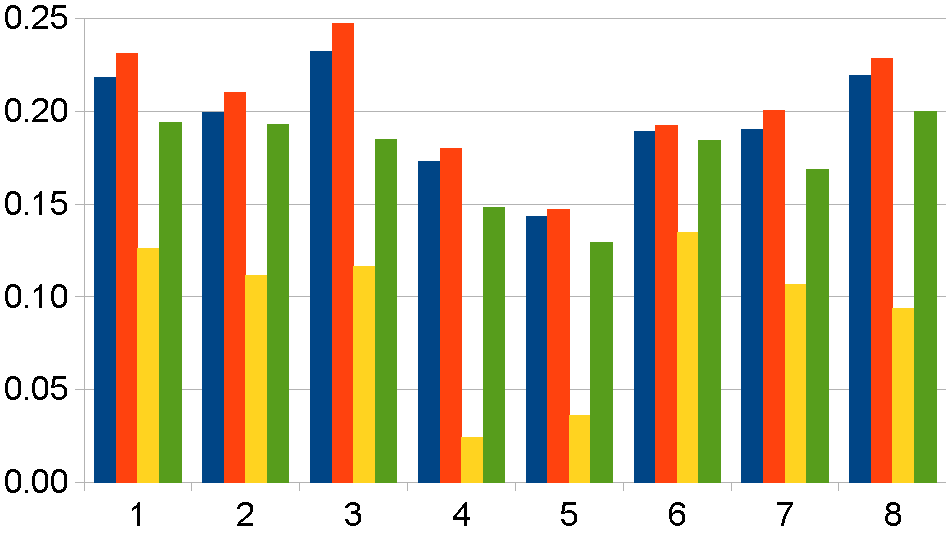
\includegraphics[page=1,width=0.9\textwidth]{graphics/tfm_results}};
        \node[below=of img, node distance=0cm, yshift=1cm,font=\color{black}] {TREC Track};
        \node[left=of img, node distance=0cm, rotate=90, anchor=center,yshift=-0.7cm,font=\color{black}] {Mean Average Precision};
    \end{tikzpicture}
    \begin{center}
        \begin{tabular}{ c c c c }
            \tikz\draw[dblue,fill=dblue] (0,0) rectangle (1.5ex, 1.5ex); No expansion
            \tikz\draw[dorange,fill=dorange] (0,0) rectangle (1.5ex, 1.5ex); Relevance feedback 
            \tikz\draw[yellow2,fill=yellow2] (0,0) rectangle (1.5ex, 1.5ex); QE
            \tikz\draw[green2,fill=green2] (0,0) rectangle (1.5ex, 1.5ex); tf-merging
        \end{tabular}
    \end{center}
    
\end{figure}

% \subsection{Hyponym Query Drift}
Let us inspect TREC-6 query 40, \textit{``land mine ban''}, to see what is really happening. With no query expansion, the AP (Average Precision) is 0.0805, with QE, the AP is 0.0014, and with tf-merging, the average precision is 0.0984. This query was chosen as QE clearly has a huge negative impact on this query, and tf-merging has a small positive effect. 

WordNet provides 180 hyponyms for the 3 query terms; 9 examples can be seen in Table \ref{example-query}. Some of these hyponyms like \textit{``ground emplaced mine''} appear relevant to the initial query. However, other terms like \textit{``goldmine''} are clearly irrelevant and could very easily cause query drift. Problematically, WordNet does not disambiguate polysemes and homographs, e.g.\ ``mine'' the explosive and ``mine'' the excavation site are conflated. More importantly, however, there are 153 expansions for the term ``land''. Hence, over 80\% of the modified query terms are either ``land'' or a hyponym of ``land'', this causes the query to drift towards land-ness, so documents exclusively about ``land'' are over boosted in the rank. Thirdly, many hyponyms for ``land'' are geographic labels and proper nouns, and proper nouns are known to cause query drift \cite{vechtomova2004use}.

%Using hypernym\textquotesingle s on Trec-6 query 14 improved from 0.0014 to 0.0102, a factor of 7.2 higher.
\begin{table}[h]
    \centering
    \small
    \begin{tabular}{|l|r|l l l|}
        \hline
        Query term & Expansions & \multicolumn{3}{c|}{Some example expansions} \\
        \hline
        \small
        land & 153 & crash land	& farmland 	& no man's land \\
        mine & 18  & goldmine		& booby trap 	& ground emplaced mine \\
        ban  & 9   & embargo		& rusticate 	& cease and desist \\
        \hline
    \end{tabular}
        \caption{Expansion hyponyms, TREC-6 query 40}
    \label{example-query}
\end{table}

With tf-merging, the query's retrieval performance was better than QE (and better than no expansion) as the excessive amount of ``land'' expansions did not cause query drift.

\subsection{Antonyms}
Our results showed that using antonyms as a source of expansion terms improves precision almost as often as synonyms. This initially seems counterintuitive as surely including the exact opposite of the query will retrieve the exact opposite results. However, this is not the case as antonyms can cause vocabulary mismatch just as synonyms can because you can describe something through its negation. The two sentences below are not strictly identical, but they convey a similar sense.

\begin{center}
    \textit{``I am \textbf{short}''}
    
    \textit{``I am \textbf{not tall}''}
\end{center}

Many antonyms are interdependent with their antonymous pair as each cannot exist without the other, e.g.\ the concept of \textit{``tallness''} depends on the concept of \textit{``shortness''}, as \textit{``shortness''} depends on the concept of \textit{``tallness''}. You cannot define one without defining the other. George Orwell also described this linguistic observation.

\begin{center}
    \textit{``what justification is there for a word which is simply the opposite of some other word? A word contains its opposite in itself. Take "good", for instance. If you have a word like "good", what need is there for a word like "bad"? "Ungood" will do just as well."}
    \\ --- George Orwell, 1984
\end{center}

Orwell's proposal to abolish antonyms was not sincere. It was part of \textit{newspeak}, a satirical spin on government censorship by means of \textit{reductio ad absurdum}.

Indeed, a common method to automatically find antonymous pairs is co-occurrence analysis \cite{JusteonKatz1991, justeson1991co}. The same method discussed previously that constructs statistical thesauri—the same method which finds synonymous pairs. According to the WordNet documentation, \textit{``direct antonyms''} are \textit{``a pair of words between which there is an associative bond resulting from their frequent co-occurrence''}, i.e.\ they have probably use co-occurrence analysis to identify antonyms.

% PROBLEM WITH WORDNET 
% Following a chain of antonmyms we arrive at a word which is unrelated to the first item in the chain,
% LEFT - RIGHT - WRONG - CORRECT

% Table \ref{tfmmap} shows the MAP of each TREC track using different query expansion techniques. The bold entries indicate an improvement over doing nothing. Rocchio's relevance feedback method shows that standard query expansion can consistently improve the mean average precision (MAP). However when using a general-purpose thesaurus (Roget/WordNet), standard query expansion degrades the MAP in all cases. These results are not unexpected. We can see that our tf-merging technique performs better than the standard approach, and occasionally performs better than doing nothing.

% %none v tf-merging	0.0027
% %none v query expansion	9.7804E-015
% %tf-mergingergin v query expansion	4.7525E-010

% \begin{table*}[t]
% \centering
% \caption{Mean Average Precision}
% \label{tfmmap}
% \begin{tabular}{|l|l|r|r|r|r|r|r|r|r|}

% \hline
% Expansion terms 				& mode	& TREC-1	& TREC-2	& TREC-3	& TREC-4	& TREC-5	& TREC-6	& TREC-7	& TREC-8 \\
% \hline
% No expansion				&				& 0.2181	& 0.1993	& 0.2324	& 0.1727	& 0.1432	& 0.1891	& 0.1905	& 0.2195 \\
% Relevance feedback				& naive		& \textbf{0.2311}	& \textbf{0.2103}	& \textbf{0.2476}	& \textbf{0.1802}	& \textbf{0.1468}	& \textbf{0.1925}	& \textbf{0.2007}	& \textbf{0.2286} \\
% \hline
% Roget				& naive		& 0.1995	& 0.1740	& 0.1945	& 0.1349	& 0.1119	& 0.1802	& 0.1853	& 0.2069 \\
% Antonym				& naive		& 0.1977	& 0.1823	& 0.2139	& 0.1411	& 0.1230	& 0.1618	& 0.1741	& 0.1977 \\
% Entailment			& naive		& 0.2153	& 0.1942	& 0.2315	& 0.1651	& 0.1311	& 0.1851	& 0.1898	& 0.2171 \\
% Hypernym			& naive		& 0.1220	& 0.0680	& 0.1139	& 0.0335	& 0.0475	& 0.1058	& 0.1011	& 0.1155 \\
% Hyponym			& naive		& 0.1258	& 0.1114	& 0.1161	& 0.0243	& 0.0362	& 0.1347	& 0.1068	& 0.0937 \\
% Meronym part		& naive		& 0.2154	& 0.1972	& 0.2250	& 0.1642	& 0.1402	& 0.1886	& 0.1896	& 0.2076 \\
% Meronym subs		& naive		& 0.2157	& 0.1839	& 0.2168	& 0.1593	& 0.1259	& 0.1860	& 0.1911	& 0.2095 \\
% Similar To			& naive		& 0.1760	& 0.1630	& 0.1754	& 0.1065	& 0.1074	& 0.1714	& 0.1715	& 0.2084 \\
% \hline
% Roget				& tf-m		& 0.2173	& 0.1986	& 0.2225	& 0.1609	& 0.1393	& 0.1877	& 0.1887	& 0.2041 \\
% Antonym				& tf-m		& 0.2157	& \textbf{0.2004}	& 0.2292	& 0.1718	& 0.1404	& 0.1851	& 0.1895	& 0.2161 \\
% Entailment			& tf-m		& 0.2180	& 0.1978	& 0.2324	& 0.1726	& 0.1319	& 0.1879	& 0.1900	& 0.2175 \\
% Hypernym			& tf-m		& 0.1446	& 0.1414	& 0.1553	& 0.1072	& 0.1012	& 0.1205	& 0.1104	& 0.1716 \\
% Hyponym				& tf-m		& 0.1940	& 0.1929	& 0.1846	& 0.1483	& 0.1292	& 0.1844	& 0.1686	& 0.1996 \\
% Meronym part		& tf-m		& \textbf{0.2190}	& \textbf{0.2022}	& 0.2307	& 0.1694	& 0.1406	& \textbf{0.1912}	& \textbf{0.1912}	& 0.2152 \\
% Meronym subs		& tf-m		& 0.2180	& 0.1993	& 0.2324	& 0.1727	& 0.1425	& 0.1891	& 0.1834	& 0.2195 \\
% Similar To			& tf-m		& 0.2075	& 0.1959	& 0.2183	& 0.1659	& 0.1301	& \textbf{0.1910}	& 0.1882	& 0.2041 \\
% \hline

% \end{tabular}
% \end{table*}




% \subsection{Speed}
% We did not focus our experiments on time efficiency but it's worth a quick mention. Relevance feedback is intrinsically slow as it require at least two passes through the search engine pipeline, and a complicated term selection process. On average, QE is about 10\% slower than no expansion, tf-mergning is about 20\% slower than no expansion, and relevance feedback is 317\% slower than no expansion. Although these results are clearly dependent on hardware and implementation which we can't guarantee are any good. Though we can say the speed differences are as expected.

%none 113.6575
%relevance feedback 324.38916666666665
%Qw 122.63833333333334
%QW 102.7425






%%%%%\section{Discussion}
%Using tf-merging may also reduce the impact of spurious terms, as their contribution is not considered 
%Since automatically selected expansion terms can be irrelevant to the original query, we reduce the effects of query drift. 

%%%%%If we could precompute the expansion terms for any given query, we could store these with the index and quickly recall them when required. Such a semantic mapping table would be \textit{almost} synonymous with a thesaurus, but not quite. An appropriate expansion term is not necessarily \textit{synonymous} with a query term, because a user generated query might not contain an important concept relevant to the information need. Users are usually unsure of the information they are requesting, which is why they are requesting it. This is why methods like blind relevance feedback are effective, because they find expansion terms which refer to concepts related to the users information need, but not contained within the initial query. 

%There are many content bearing terms that are not added to the query expansion. imprecise vocabulary.

% It may also inadvertently broaden the interpretation(s), leading to query drift, as we are not guaranteed that automatically selected expansion terms are relevant.
 %This is likely due to the fact that the vocabulary of the general-purpose thesauri we tested, do not coincide with the vocabulary of the corpus.
 %Perhaps with more adjustments a general-purpose thesaurus might be useful, but we must take the necessary precautions to prevent query drift, as they will unlikely reflect the vocabulary used in most documents collections. Specialized domain specific thesauri are recommended. 

%A thesaurus constructed specifically for a the document collection may provide better results. A corpus specific thesaurus could be done either manually, or through automatic means. Either way the vocabulary used in such a thesaurus would more likely coincide with the vocabulary of the corpus it was derived from. %










\section{Conclusions}

Our results agree with the literature. Query expansion is unreliable when using a semantic ontology (like WordNet or Roget) as a source of expansion terms. Even though WordNet 3.1 is more comprehensive, it is still not viable for na{\"i}ve query expansion. This is because WordNet is a lexical-semantic ontology that cannot disambiguate polysemous and homographic words, which leads to poor quality expansion terms, resulting in query drift.

% Relevance Feedback, which is statistical in nature and collection dependent is more reliable.
% We could also blame the fact that it's a global, collection independent source of expansion terms. 

Hyponyms (and hypernyms) are ineffective for expansion. Antonyms are surprisingly effective because they have similar linguistic properties to synonyms.

Term Frequency Merging can be implemented at index time. This would require the indexer to identify synonyms (or SynSets) across the document collection and replace them with the same term (lexical token). The benefit to this approach would be the zero cost to merge at search time. However, disambiguating polysemes and homographs would still pose an an issue.

Many other expansion models could easily implement tf-merging but unfortunately not Relevance Feedback, since its expansion terms derive from documents, not directly from individual query terms, so it is not immediately clear which expansion term should be merged with which original query term.

If the expansion terms are of poor quality, tf-merging does little to help. Our method only improves retrieval in the particular case where there is query drift caused by an uneven distribution of expansion terms, i.e.\ one query term has more expansions than another.


% The purpose of our experiments was to determine if using general-purpose thesauri for query expansion could be improved. We tested two different thesauri (Roget and Wordnet), with two different query expansion techniques. We compared standard query expansion with our proposed method that we call tf-merging.

% Our results agree with the literature, using a general-purpose thesauri appears to have potential but lacks reliability. Despite the fact that WordNet has become more comprehensive as a thesaurus, it is still not viable for QE. It \textit{can}, and frequently does, improve the precision of ad-hoc retrieval tasks, but there is still a large chance that the precision will be degraded. 

% Reformulating a query through tf-merging makes sense intuitively, as we are not biasing our search towards query terms which have more expansions. What we have proposed is straightforward and efficient, and it does not require a sophisticated language model to be implemented. Our approach of tf-merging does empirically improve general-purpose thesauri query expansion, but not enough to be competitive against other query reformulation methods.

% compare to other people's work
% Since our results indicate an improvement to thesaurus based expansion, in future work we will apply tf-merging to other query reformulation methods. The most obvious choice would be relevance feedback approaches, as their effectiveness is well established, especially the RM3 relevance model \cite{abdul2004umass}. Since tf-merging is independent of the expansion term selection process, it could easily be used to complement existing query expansion improvements. We will also test the effectiveness with other ranking functions that use TF and IDF scores.



% It is likely that tf-merging will fail to reduce the effects of query drift, when there are many discriminating spurious terms in every expansion set. But if the expansion term selection process is good, then tf-merging should be able to improve it.

% We suspect that tf-merging can reduce the negative effects of query drift, when the spurious terms are far less common than the favorable expansion terms. If the expansion term selection process is dreadful, then tf-merging will struggle to improve it by very much.


% \section{Statistics}
% Statistics
% two standard deviations from the mean
% outside the range
% but still perfectly normal
% performing the experiment 20 times, one outside the range
% this would be as expected
% now the results so far, are definitely outside the expected range
% that doesn't definitively conclude that the results have improved, or even changed, the difference could still be random noise
% but it some evidence that there is a degree of bias towards improvement
% Again, the bias isn't confirmed, unequivocally
% but it's just a failure to reject
% There is undeniable plausibility
% If I were a betting man, I would bet money on this (not too much mind you, I'm a broke Masters student)
% There is no way to confirm the results of this experiment, or increase the p value to ??? ... 100%
% Instead of inferring whether or not a user has succeeded in full-filling the information request by analysing their behaviour
